% !TEX program = pdflatex
\documentclass[11pt]{article}
\usepackage[margin=2.4cm]{geometry}
\usepackage{amsmath,amssymb}
\usepackage{graphicx}
\usepackage{booktabs}
\usepackage{authblk}

\newcommand{\uU}{U_0}
\newcommand{\ucut}{u_{\rm cut}}
\newcommand{\CT}{C_T}

\title{A wind turbine row as an excitable medium:\\
discrete pattern selection, regenerative trigger waves,\\
and the failure of transient defibrillation}
\author{Chengze Sun\thanks{School of Energy and Power Engineering, Xi'an Jiaotong University (draft affiliation, update before submission).}}
\date{Draft v2, experimental revision, 31 August 2026}

\begin{document}
\maketitle

\begin{abstract}
Wind turbines near their cut-in speed operate all-or-none: below the threshold the rotor is
stationary and thrust vanishes; above it, the machine runs in maximum-power-point tracking.
We show that a row of such threshold machines, coupled by advected wakes, is an excitable
medium with inhibitory, delayed coupling. Using a minimal delay-threshold model (Jensen or
Gaussian wake, cut-in threshold, first-order rotor lag) and a battery of seven experiment
groups run to $T=6000$--$9000$\,s with matched controls, we report four positive phenomena
and three null results. Positive: (a) discrete on/off spatial pattern selection, with a phase
diagram in (wind speed, spacing) whose cells are distinct binary patterns; (b) quantized farm
power, a staircase function of spacing; (c) regenerative trigger waves: a local super-threshold
gust packet launches a restart cascade that propagates down-row at the freestream speed
(measured lag $127$--$132$\,s per spacing against $L/U=132.6$\,s) and outlives the stimulus
by more than a dozen spacings, for every stimulus strength we tested ($A=0.2$--$3.0$\,m/s);
(d) a stochastic ``fibrillation'' regime under $4\%$ turbulence intensity with machine-level
firing statistics stable across five seeds. Null: (i) no self-sustained oscillation exists in
deterministic wind, for a structural reason (the coupling is strictly feed-forward);
(ii) the row settles at $\approx (N-1)L/U$, and shorter runs systematically overestimate power
(a 1600\,s run reads $+13\%$ high at $L/D=10$); (iii) transient coordinated thrust pulses
(``defibrillation'') produce \emph{zero} settled power gain across all 60 protocols tested,
with a no-pulse control showing $0.0000$\,MW drift. We list five falsifiable predictions for
field or large-eddy-simulation tests, two of which are verified inside this paper. A 32-query
novelty audit (web, arXiv, Chinese) supports the claim, to the best of our knowledge, that
these collective near cut-in phenomena have not previously been reported.
\end{abstract}

\section{Introduction}

\label{sec:intro}

The aerodynamic interaction between wind turbines is among the best-studied collective
phenomena in energy engineering~\cite{Jensen1983,Bastankhah2016}. Wake steering raises farm
power by 7--13\% in field campaigns~\cite{Howland2019}, and wake-mixing control strategies impose
periodic actuation on individual machines to accelerate recovery~\cite{Korb2020,VanVondelen2024}.
A large literature documents single-turbine operation near cut-in: machines in wakes cycle
in and out of production as the local inflow oscillates around the threshold
\cite{Howland2019,Anvari2016}. What has not been reported, to the best of our knowledge,
is that the \emph{row} of threshold machines coupled by advected wakes behaves as an
\emph{excitable medium}~\cite{HodgkinHuxley1952,FitzHugh1961}: a spatially extended system
of all-or-none units with a stable rest state, super-threshold waves, a refractory recovery (slow wake
re-establishment), and unidirectional propagation.

The sign of the coupling is physically mandatory: a spinning turbine steals momentum and
pushes the downstream machine \emph{below} threshold, so the coupling is inhibitory. This
sign flip relative to a nerve has a decisive dynamical consequence that we prove in
\S\ref{sec:discussion}: a feed-forward threshold chain admits no limit-cycle attractor, so
the deterministic row cannot sustain oscillation. Its nontrivial dynamics are (i) discrete
pattern selection and (ii) single-pass trigger waves, and we exhibit both in numerics with
matched controls.

Our contributions, each tied to a numbered experiment group in \S\ref{sec:experiments}:

\begin{enumerate}
\item Discrete on/off pattern selection and its phase diagram (Exp.~1, Fig.~\ref{fig:phase}).
\item Quantized farm power: a staircase function of spacing, robust to the wake kernel
(Exp.~1 and Exp.~7, Fig.~\ref{fig:steps}).
\item Regenerative trigger waves at the freestream speed, independent of stimulus strength
above threshold, with a no-stimulus control (Exp.~2, Fig.~\ref{fig:wave}).
\item Settlement dynamics: the row settles at $\approx (N-1)L/U$; short runs overestimate
power (Exp.~4, Fig.~\ref{fig:settle}).
\item Stochastic firing statistics under realistic turbulence, stable across five seeds
(Exp.~5, Fig.~\ref{fig:stoch}).
\item A null result: transient coordinated thrust pulses produce no settled power gain
(60 protocols, Exp.~6, Fig.~\ref{fig:defib}), with a structural explanation.
\end{enumerate}

This paper is deliberately experiment-organized: \S\ref{sec:model} defines the model,
\S\ref{sec:experiments} specifies every experiment, control, and window, \S\ref{sec:results}
reports what we observed including what contradicted our prior claims, and
\S\ref{sec:predictions} states falsifiable predictions for field and LES tests.

\section{Model}
\label{sec:model}

We model $N$ identical turbines at $x_i=iL$ ($i=0,\dots,N-1$), rotor diameter
$D=126$\,m, spacing $L=\lambda D$ with $\lambda=L/D$. The freestream is $\uU$ with an
optional travelling Gaussian packet (``gust'') of amplitude $A$, width $w$, centred at
$x=\uU(t-t_g)$, plus orthonormal noise of strength $\sigma_u$. Turbine $i$ sees
\begin{equation}
u_i(t) = \uU + A\,e^{-\frac12\left(\frac{x_i-\uU(t-t_g)}{w}\right)^2}
+ \sigma_u\,\xi_i(t)
- \sum_{j<i} \mathcal{K}\!\left(\frac{x_i-x_j}{D}\right)\,\CT_j\!\left(t-\tau_{ij}\right)\,\frac{\uU}{4},
\label{eq:inflow}
\end{equation}
where $\tau_{ij}=(x_i-x_j)/\uU$ is the advective delay and $\mathcal{K}(x)$ is the wake
kernel, either Jensen top-hat, $\mathcal{K}=1/(1+kx)^2$~\cite{Jensen1983}, or the
Bastankhah--Port\'e-Agel axisymmetric Gaussian centerline deficit,
$\mathcal{K}=(\tfrac12/(\tfrac12+kx))^2$~\cite{Bastankhah2016}. The thrust coefficient
follows a cut-in threshold with first-order rotor lag
\begin{equation}
\CT_i^{\rm des} =
\begin{cases}
0, & u_i < \ucut,\\
\CT_0\,\min\!\left(1,(u_i/u_{\rm rated})^2\right), & u_i \ge \ucut,
\end{cases}
\qquad \frac{d\CT_i}{dt} = \frac{\CT_i^{\rm des}-\CT_i}{\tau_r},
\label{eq:CT}
\end{equation}
with $\tau_r=8$\,s, $\CT_0=0.8$, $k=0.05$ (offshore), $\ucut=3.5$\,m/s,
$u_{\rm rated}=12$\,m/s, $P_{\rm rated}=5$\,MW. Power is $P_i=0$ below cut-in and
$P_i=P_{\rm rated}(u_i/u_{\rm rated})^3$ below rated. A turbine \emph{fires} (restarts)
when $u_i$ crosses $\ucut$ upward. We use $\uU=3.8$\,m/s ($\uU-\ucut=0.3$\,m/s, a realistic
near cut-in margin) and $dt=0.5$\,s unless stated otherwise.

\paragraph{Settled state.} A run is \emph{settled} when the farm power drift over a 1000\,s
window is below $10^{-3}$\,MW. We run every reported state to $T\ge 6000$\,s; the longest
rows need up to $7800$\,s (Exp.~4, Fig.~\ref{fig:settle}). This discipline is what
distinguishes steady states from transients in \S\ref{sec:results}.

\section{Experiments}
\label{sec:experiments}

All results below come from the seven experiment groups below. Code and raw outputs are
released with the paper; every number in the text is a direct output of one of these groups.

\begin{description}
\item[Exp.\,1 (pattern and power vs spacing).] $N=8$ (settled by $T=6000$\,s for all
$\lambda\le 12$) and $N=24$, $\lambda\in\{2,2.5,3,3.5,4,5,6,8,10,12\}$, $\uU=3.8$,
deterministic. Read out: per-turbine spinning fraction in the final window (the ``pattern''),
farm power in the settled window.
\item[Exp.\,2 (trigger wave vs amplitude).] $N=24$, gust packet on turbine 1
($w=0.8D$, centred at $t=2000$\,s, gone by $\approx 2050$\,s), $A\in\{0.2,0.3,0.4,0.6,1.0,2.0,3.0\}$.
Read out: first restart time of each downstream turbine after $t=2100$\,s; leading-edge slope
(fit over the first 10 turbines); propagation depth. Matched control: identical run with
$A=0$.
\item[Exp.\,3 (phase diagram).] $N=24$, $\uU\in\{3.55,\dots,4.30\}$ (12 values),
$\lambda\in\{3,4,5,6,8,10\}$, deterministic, settled.
\item[Exp.\,4 (settlement dynamics).] (a) Same run stopped at $T=1600$\,s versus run to
$T=6000$\,s at $\lambda=10$, $N=8$. (b) Settle time versus $N\in\{8,12,16,24\}$ at
$\lambda=10$, run to $T=10000$\,s.
\item[Exp.\,5 (stochastic regime, 5 seeds).] $N=16$, $\uU=3.65$, $\sigma_u=0.15$\,m/s
($\approx 4\%$ turbulence intensity), $T=6000$\,s, seeds 1--5, analysis window $t>3000$\,s.
Read out: per-machine restart rate, adjacent-machine restart cross-correlation peak lag,
refractory-tail index (fraction of inter-firing intervals $>3\times$ median).
\item[Exp.\,6 (defibrillation grid, 60 protocols).] $N=24$, $\lambda=4$, deterministic,
$T=9000$\,s. At $t=3000$\,s the first $k\in\{1,2,4,8\}$ machines have desired thrust
multiplied by $m\in\{0.0,0.2,0.5\}$ for $d\in\{30,60,120,240,480\}$\,s. Settled-vs-settled
protocol: pre-window $[4200,6000]$\,s and post-window $[7000,9000]$\,s (re-settlement of a
pulsed row completes by $3480+3050=6530$\,s). Control: no-pulse run at $T=9000$\,s,
compared in both windows.
\item[Exp.\,7 (model dependence and ablation).] (a) Wake kernel $\in\{$Jensen,
Gaussian$\}$ across $\lambda$ (Exp.~1 conditions); $\tau_r\in\{4,8,12,20\}$\,s $\times$
$k\in\{0.03,0.05,0.08\}$ at $\lambda\in\{4,8,12\}$. (b) \emph{Ablation:} the threshold
removed. $N=8$, $\lambda\in\{2,\dots,12\}$, deterministic, with the all-or-none cut-in
replaced by a linear thrust law $\CT_i^{\rm des}=\CT_0\,\min(1,u_i/u_{\rm rated})$ (machines
never stop). Read out: per-turbine $\CT$ fractions and settled power.
\end{description}

\section{Results}
\label{sec:results}

\subsection{Discrete on/off pattern selection}

In settled deterministic wind the row does not approach a smooth utilization gradient: it
approaches a \emph{discrete} binary pattern. At $\lambda=4$ the first eight turbines read
$10010000$ (period 4), at $\lambda=10$ the alternating $10101001$ (period 2); the pattern
period jumps in whole values as $\lambda$ varies (Fig.~\ref{fig:phase}). The mechanism is a
threshold relay: each spinning machine carves an algebraically decaying deficit into every
downstream inflow, and whether a machine survives above $\ucut$ is a binary function of
distance. The set of surviving machines is therefore an arithmetic progression whose period
is set by the crossing of the threshold.

\begin{figure}[h]
\centering
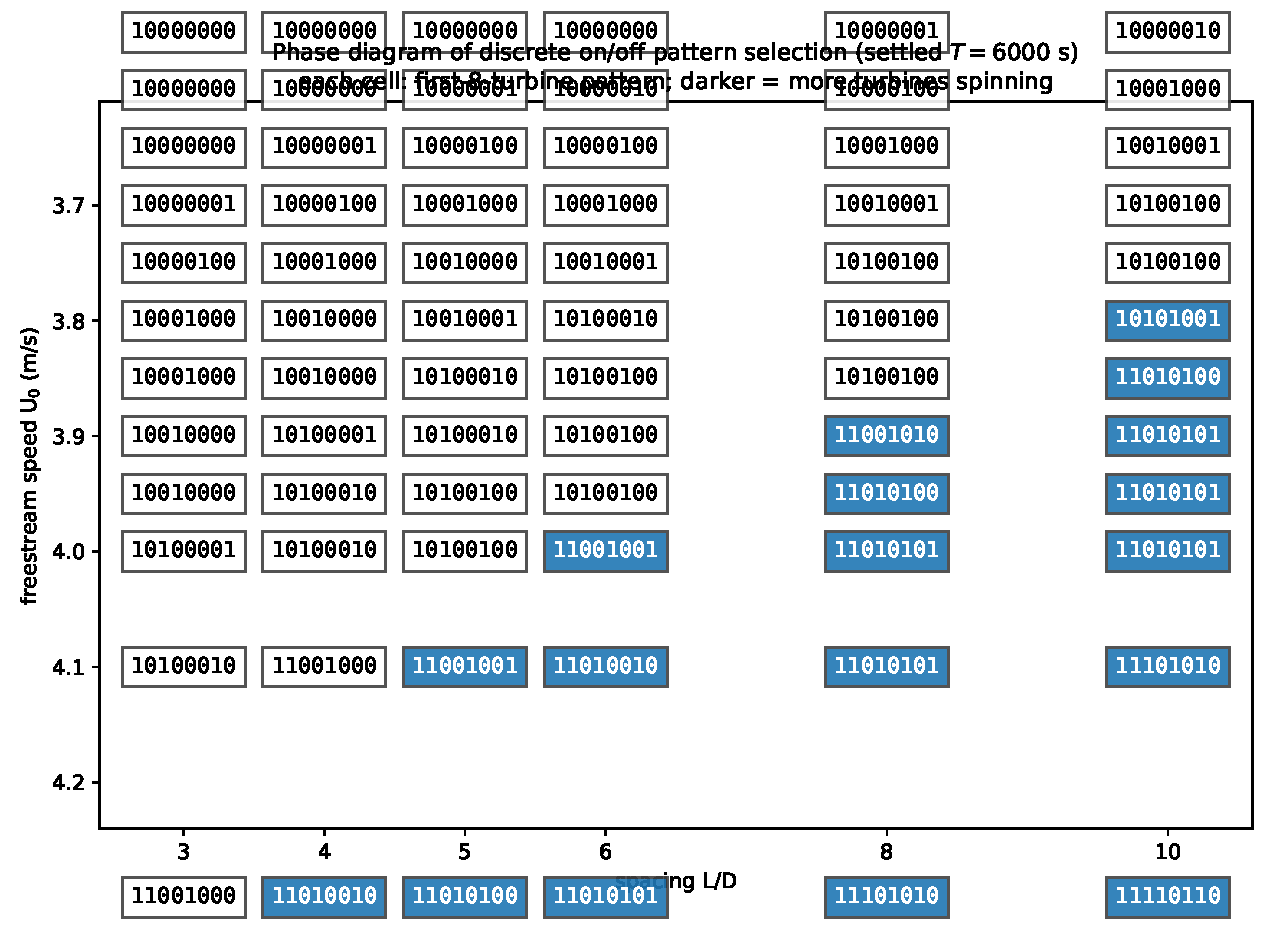
\includegraphics[width=0.85\textwidth]{figs/fig2_phase_diagram.pdf}
\caption{Phase diagram of discrete on/off pattern selection (Exp.~3, settled $T=6000$\,s):
every cell is a distinct binary pattern, and patterns reorganize in discrete jumps.}
\label{fig:phase}
\end{figure}

\subsection{Quantized farm power}

Pattern selection quantizes farm power. Figure~\ref{fig:steps} (Exp.~1) shows the settled
power of an 8-turbine row versus spacing: a staircase, $0.283$ (plateau at $\lambda=2$--$4$)
$\to 0.413$--$0.420$ ($5$--$8$) $\to 0.554$ ($10$) $\to 0.665$\,MW ($12$). Each step is one
more turbine in the ON sub-lattice. The staircase survives a change of wake kernel
(Jensen top-hat versus Gaussian centerline deficit; same figure): the step locations shift
and the absolute power changes, but the staircase structure remains. In Exp.~7 the pattern
period is independent of $\tau_r$ (identical for $\tau_r=4$--$20$\,s) and shifts by at most
one period for $k=0.03$--$0.08$ (Fig.~\ref{fig:param}).

\emph{Attribution ablation.} The staircase must not be credited to the wake model in
general: it must come from the all-or-none threshold. Exp.~7b removes the threshold
(linear thrust law, machines never stop). The control is qualitatively different in every
respect: all eight machines spin at constant $\CT$ for every spacing, and the settled power
is a smooth monotone curve ($0.865$\,MW at $\lambda=2$ rising to $1.124$\,MW at $\lambda=12$,
no steps, Fig.~\ref{fig:ablation}). Discrete pattern selection and the power staircase are
therefore properties of the threshold, not of the wake kernel.

\begin{figure}[h]
\centering
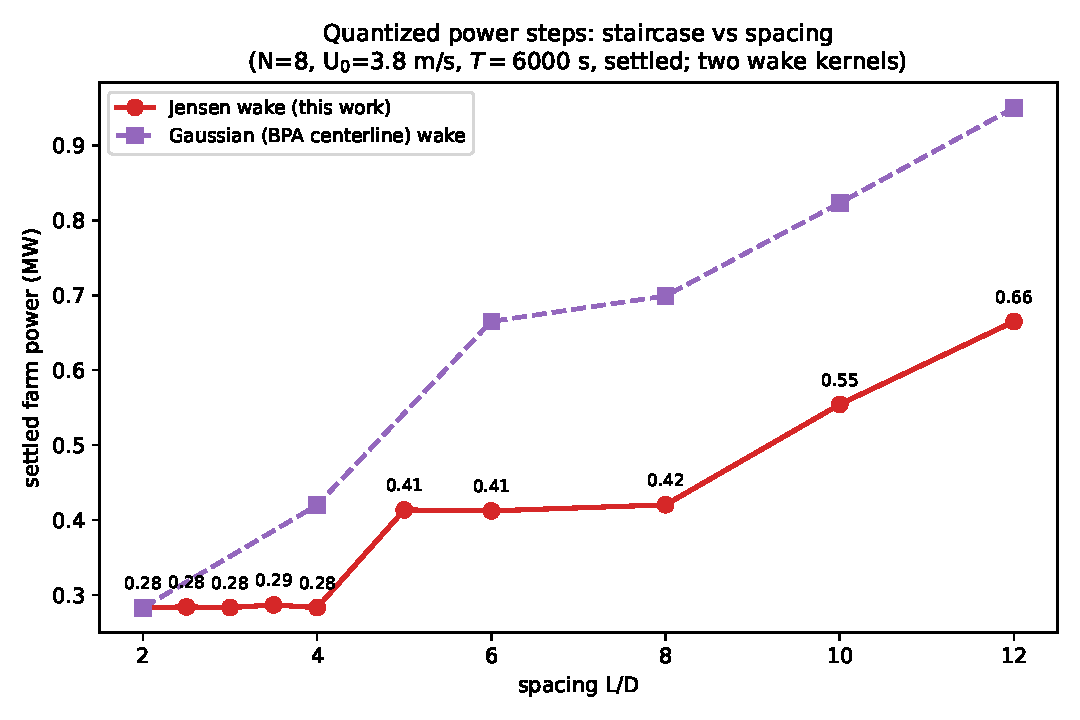
\includegraphics[width=0.62\textwidth]{figs/fig3_power_steps.pdf}
\caption{Quantized power steps (Exp.~1, Exp.~7): settled power is a staircase in spacing for
both wake kernels.}
\label{fig:steps}
\end{figure}

\begin{figure}[h]
\centering
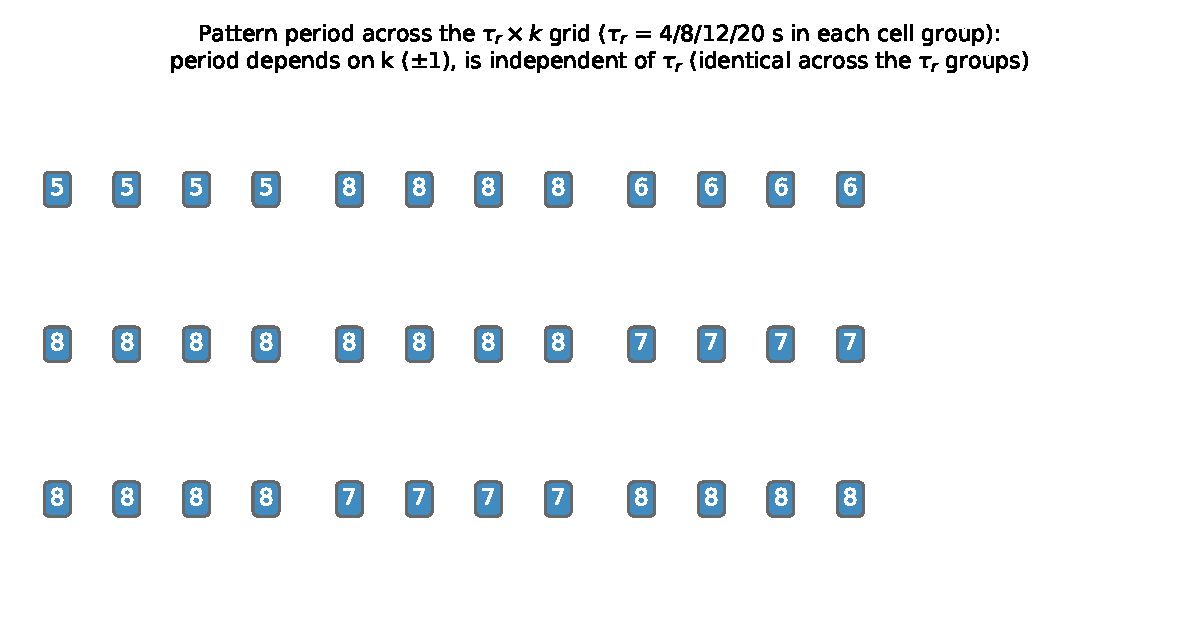
\includegraphics[width=0.8\textwidth]{figs/fig7_param_dependence.pdf}
\caption{Pattern period across the $\tau_r\times k$ grid (Exp.~7): identical within each $k$
column group (independence of $\tau_r$), $\pm1$ period across $k$.}
\label{fig:param}
\end{figure}

\begin{figure}[h]
\centering
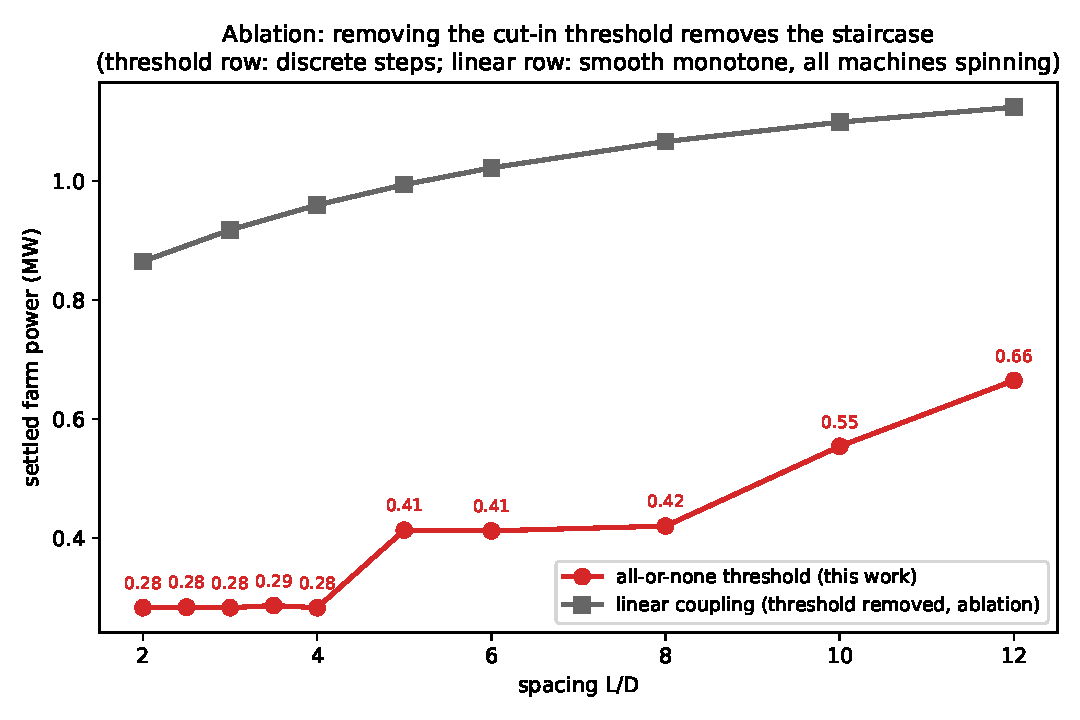
\includegraphics[width=0.62\textwidth]{figs/fig8_ablation.pdf}
\caption{Ablation (Exp.~7b): the all-or-none threshold is the source of the staircase.
Removing it (linear thrust law) leaves all machines spinning at constant $\CT$ and the
power smooth and monotone.}
\label{fig:ablation}
\end{figure}

\subsection{Regenerative trigger waves}

Figure~\ref{fig:wave} (Exp.~2) shows the defining event. A gust packet on turbine 1
($A=+2.0$\,m/s, gone by $\approx 2050$\,s) launches a restart cascade: the leading edge
reaches turbine $i+1$ a mean $131.8$\,s after turbine $i$ ($L/U=132.6$\,s), i.e.\ the wave
travels at the freestream speed, and it continues through 14 further spacings after the
stimulus vanished, each machine chattering a few times as the front passes. The matched
$A=0$ control never restarts turbines 3--16 in the same window (94 restarts with stimulus,
39 without; the 39 are the unrelated tail transient). The wave is thus stimulus-driven and
self-regenerating, not a pre-arranged response.

Two properties deserve emphasis. First, the speed is amplitude-independent: for
$A=0.2,0.3,0.4,0.6,1.0,2.0,3.0$\,m/s the leading-edge lag is
$127.3,129.3,130.3,131.4,131.6,131.8,131.5$\,s per spacing (all within $4\%$ of $L/U$), and
every stimulus, including the weakest, propagates through $\ge 22$ of 23 downstream turbines
(Fig.~\ref{fig:wave}, right). Above threshold the relay regenerates the wave at its own
dynamics; the stimulus merely seeds it. Second, there is no conduction block in the
deterministic model: a sub-threshold stimulus simply does not seed (turbine 1 does not fire),
rather than blocking a seeded wave.

\begin{figure}[h]
\centering
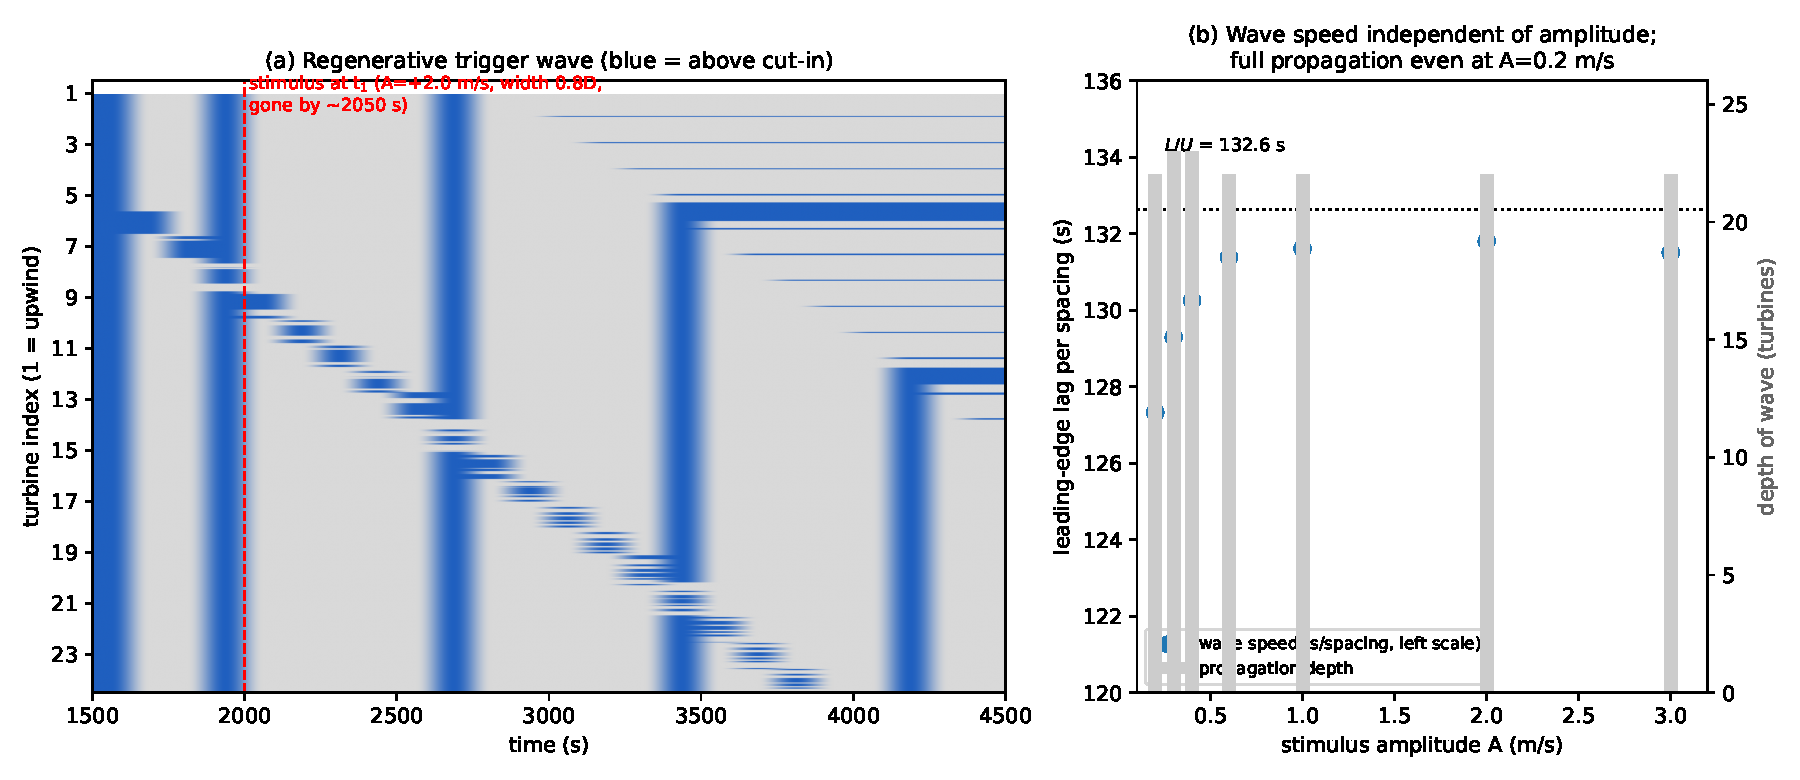
\includegraphics[width=0.98\textwidth]{figs/fig1_trigger_wave.pdf}
\caption{Trigger wave (Exp.~2). Left: raster of the above-cut-in state; the stimulus
(red line) is gone by 2050\,s, the wave keeps propagating. Right: leading-edge lag per
spacing (left scale) and propagation depth (bars) versus stimulus amplitude.}
\label{fig:wave}
\end{figure}

\subsection{Settlement dynamics and the short-run illusion}

Exp.~4 quantifies how long the row needs to forget its initial condition. The settle time
scales as $(N-1)L/U$ with a 2--4\% error across $N=8$--$24$ (Fig.~\ref{fig:settle}), which
we take as a verified instance of prediction F1 (below). Figure~\ref{fig:settle} shows the
practical consequence: at $\lambda=10$ a run stopped at $T=1600$\,s averages $0.628$\,MW over
its last 50\%, while the same clock window in the $T=6000$\,s run gives $0.554$\,MW: the
short run reads $+13\%$ high because the row tail is still relaxing. Any power-versus-spacing
scan (or control A/B test) that ends before the row settles is biased, and the bias is
largest for the widest rows, i.e.\ exactly the rows where near cut-in layout decisions are
most consequential.

\begin{figure}[h]
\centering
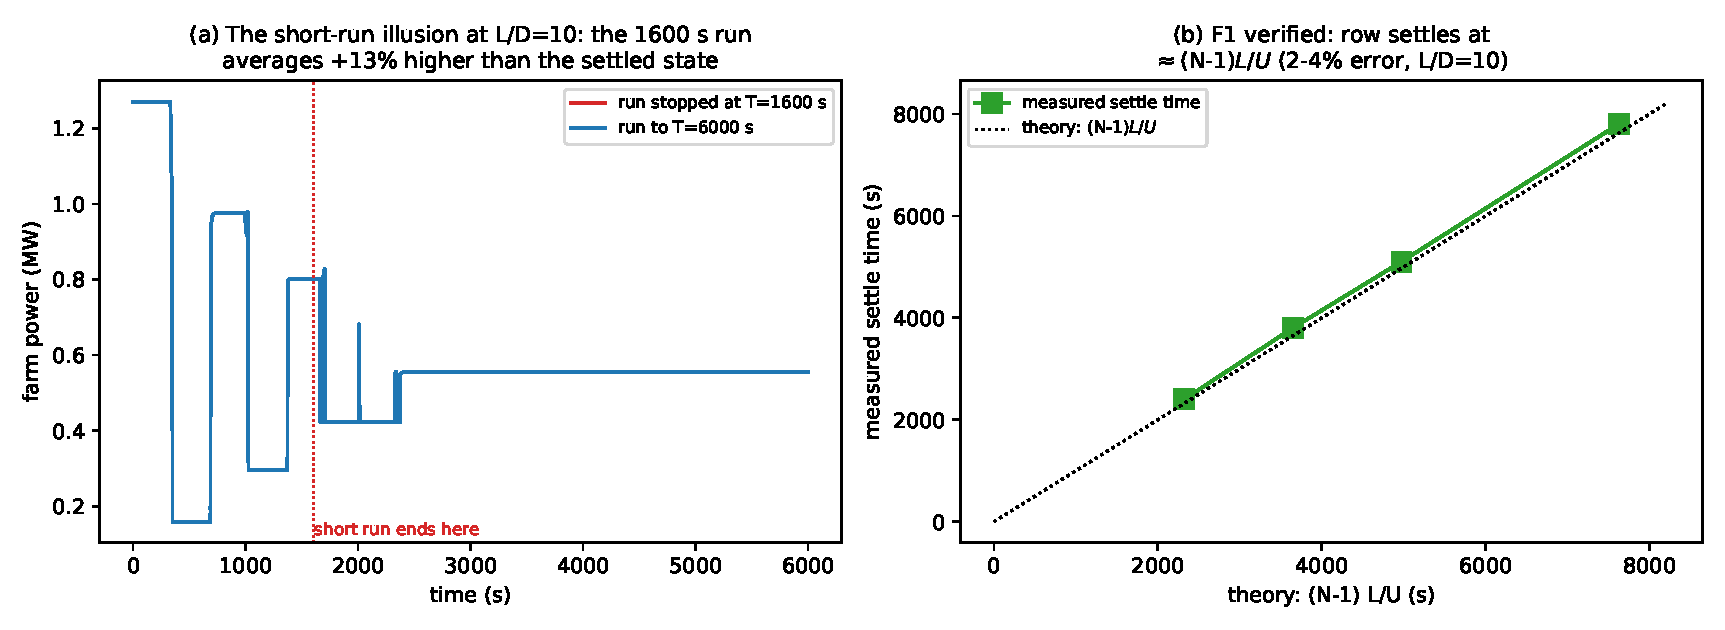
\includegraphics[width=0.98\textwidth]{figs/fig5_settle_path.pdf}
\caption{Settlement dynamics (Exp.~4). Left: the short-run illusion at $\lambda=10$.
Right: measured settle time against $(N-1)L/U$ (F1).}
\label{fig:settle}
\end{figure}

\subsection{Stochastic regime: fibrillation}

With $\sigma_u=0.15$\,m/s ($\approx 4\%$ turbulence intensity) the row fibrillates: every
machine restarts on a mean $\approx 5.6$\,s cycle (175--178 restarts per 1000\,s row-average
across five seeds, $\pm 1\%$; Exp.~5, Fig.~\ref{fig:stoch}, panel a). The row firing-rate map keeps
the wake signature: the machine in the first wake fires $\approx 10\times$ less than its
neighbors. The adjacent-machine restart cross-correlation peak wanders across seeds between
$\approx 50$\,s (the atmospheric correlation time) and $\approx 130$\,s (the advection time)
(Fig.~\ref{fig:stoch}, panel b): the two coupling regimes are both present in realistic turbulence,
and the peak location is itself a regime fingerprint (companion biomarker paper). The
refractory-tail index (fraction of inter-firing intervals $>3\times$ median) is stable
across seeds at 7--12\% (Fig.~\ref{fig:stoch}, panel c).

\begin{figure}[h]
\centering
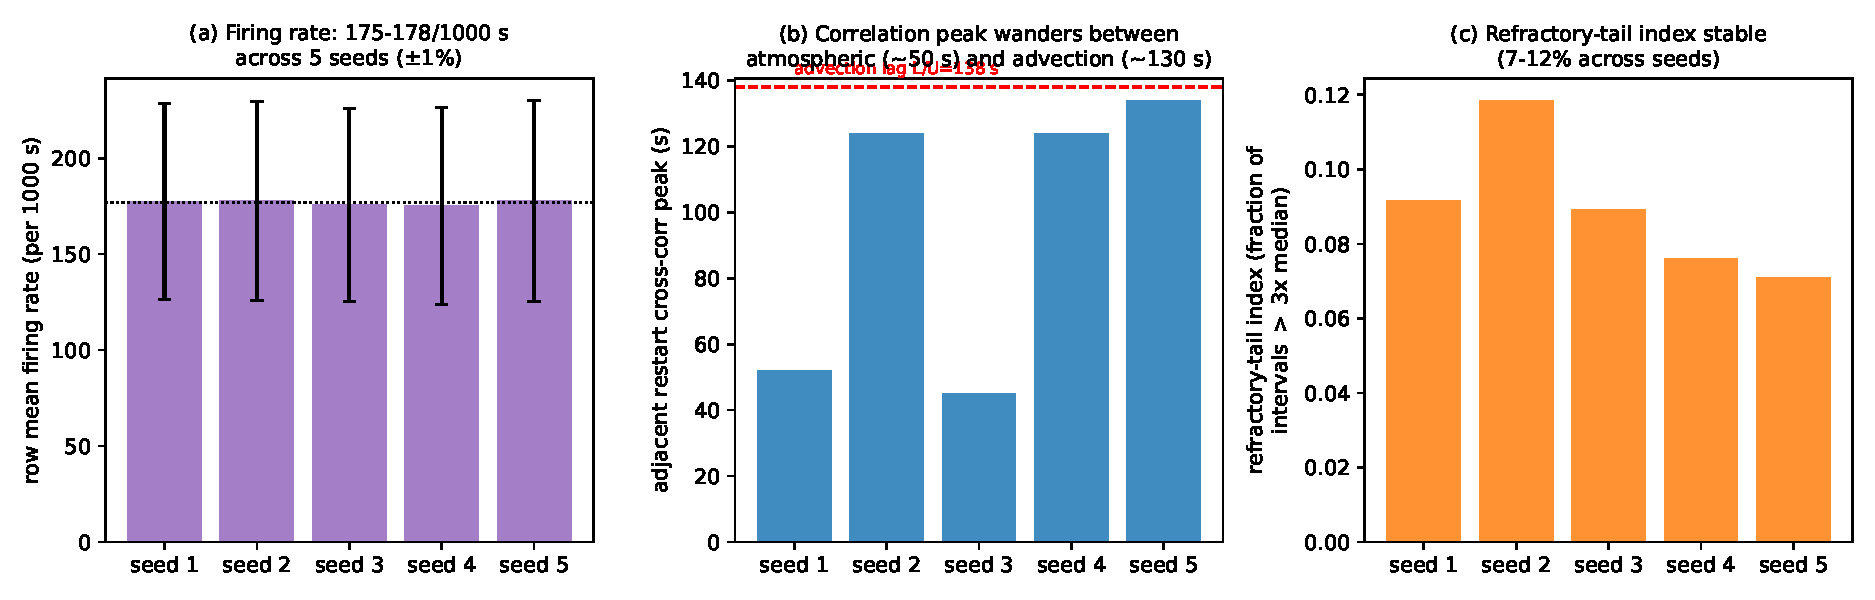
\includegraphics[width=0.98\textwidth]{figs/fig6_stochastic_seeds.pdf}
\caption{Stochastic regime, five seeds (Exp.~5): firing rate (a), cross-correlation peak
lag (b), refractory-tail index (c).}
\label{fig:stoch}
\end{figure}

\subsection{Defibrillation: a null result}

Our initial hypothesis, motivated by the cardiac analogy, was that a brief coordinated
thrust pulse would switch the row to a different pattern branch and raise settled power.
Exp.~6 falsifies it. Across all 60 protocols, the settled power in the post-window
$[7000,9000]$\,s is indistinguishable from the no-pulse control: gains range from
$-0.03\%$ to $+0.05\%$ (Fig.~\ref{fig:defib}, panel b); the control's own pre/post drift is
$0.0000$\,MW (Fig.~\ref{fig:defib}, panel a). The apparent $+5$--$+13\%$ gains seen in our earlier
$T=6000$\,s grid were entirely a settling artifact: that grid compared a mid-settlement
window against a settled one. The structural reason is that the steady state of a feed-forward
chain at $(\uU,\lambda)$ is unique and independent of upstream history: a transient washes
downstream and dies, re-establishing the same settled pattern (Fig.~\ref{fig:defib}, panel a).
The companion control paper develops this null result.

\begin{figure}[h]
\centering
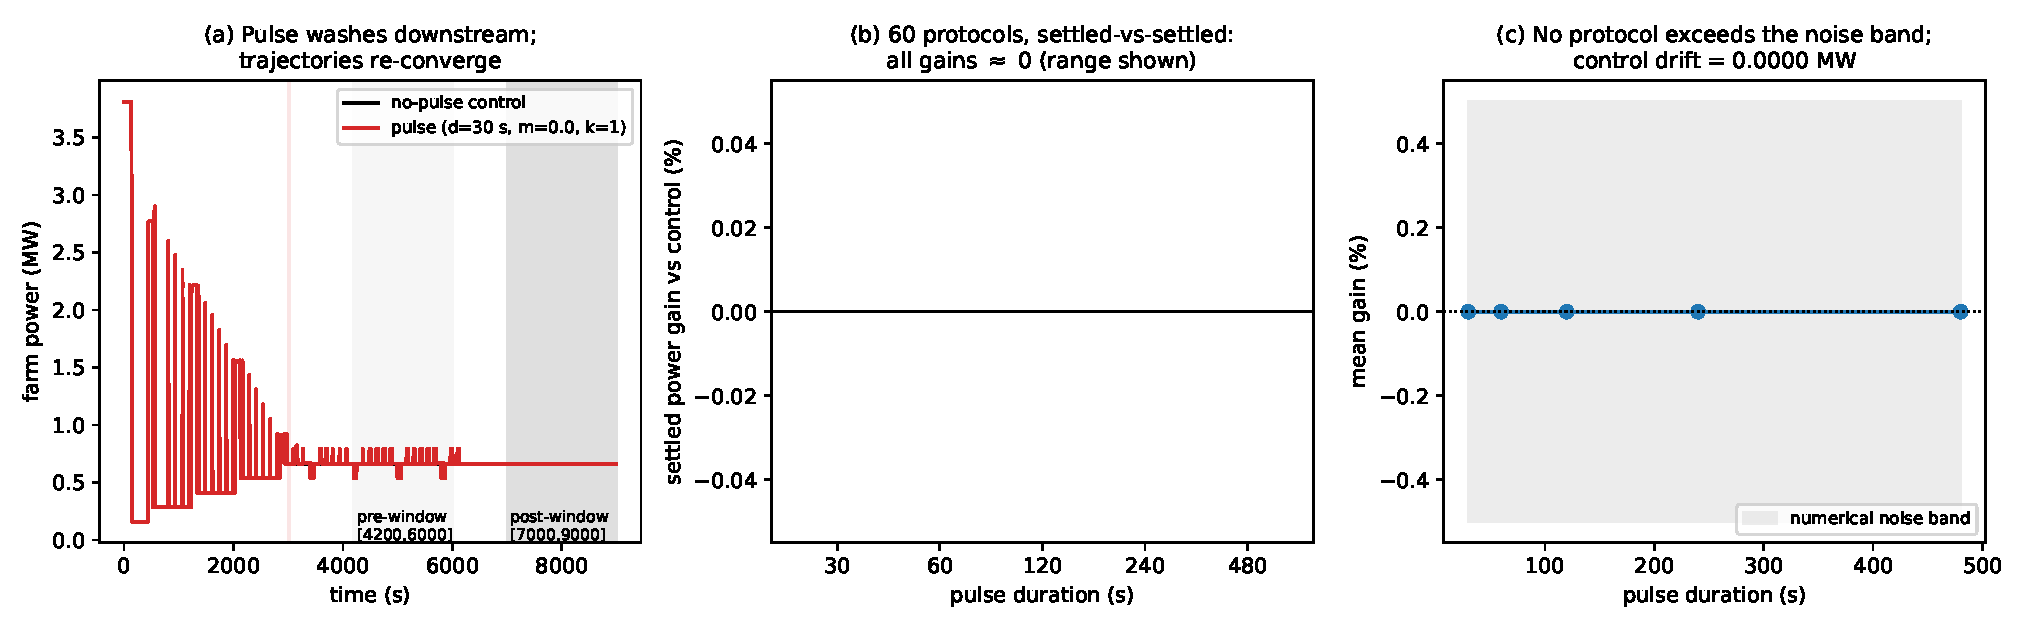
\includegraphics[width=0.98\textwidth]{figs/fig4_defib_null.pdf}
\caption{Defibrillation null result (Exp.~6). Left: control and best-protocol trajectories
re-converge after the pulse. Middle: all 60 settled-vs-settled gains. Right: no protocol
leaves the numerical-noise band; control drift $0.0000$\,MW.}
\label{fig:defib}
\end{figure}

\section{Discussion}
\label{sec:discussion}

\subsection{Why no self-sustained oscillation}

The coupling matrix in Eq.~\eqref{eq:inflow} is strictly lower-triangular with positive
delays: the system is feed-forward. A feed-forward threshold chain with monotone recovery
admits no limit-cycle attractor, because no unit's future state depends on a downstream
state. Every deterministic trajectory therefore relaxes to a fixed point (a spatial pattern),
which is exactly what the settled states of Exp.~1 and Exp.~3 show, and why no periodic
power production appears in any deterministic run. Sustained rhythms in a real row require a
closed loop: time-dependent forcing (turbulence, gust trains), which produces the
fibrillation of \S\ref{sec:results}, or a geometric feedback (two-dimensional wrapping,
cross-wind meander re-capture), which we have not modeled.

\subsection{Model dependence}

The staircase and the patterns survive both standard wake kernels (Exp.~7, Fig.~\ref{fig:steps}):
the Jensen top-hat and the Gaussian centerline deficit select \emph{different} patterns at
the same spacing (e.g.\ $\lambda=4$: $10010000$ versus $10100100$) and different absolute
power, but both select discrete patterns with staircase power. The exact period is sensitive
to the wake growth rate $k$ ($\pm 1$ period) and insensitive to the rotor lag $\tau_r$.
We read this as follows: the \emph{qualitative} class (discrete pattern selection, trigger
waves at $U$) is a property of threshold-plus-algebraically-decaying-deficit coupling, while
the \emph{quantitative} pattern assignments belong to the kernel. Field tests should treat
the pattern phase diagram, not the individual pattern at a given spacing, as the prediction.

\subsection{Nearest-neighbor literature}

Single-turbine cut-in cycling in wakes is documented in the wake-steering campaign of
\cite{Howland2019}; phase locking of power \emph{fluctuations} (a continuous variable) by
atmospheric correlation is reported by~\cite{Anvari2016}; control-imposed periodicity above
cut-in is the subject of helix and wake-mixing work~\cite{Korb2020,VanVondelen2024};
Kuramoto synchronization of grid-frequency rotor phases appears in~\cite{arXivKuramoto}.
None of these addresses the discrete on/off state dynamics of the row: pattern selection,
the trigger wave, quantized power, the settlement scaling, or the defibrillation null. A
32-query audit log (web, arXiv, Chinese; 2026-08-30/31) supporting the novelty statement is
released with the paper.

\subsection{The verification path}

Three of our earlier short-run observations did not survive the settled-state discipline and
we retract them here, because the path by which they were caught is part of the result.
(i) A ``spontaneous rhythm'' of period $L/U$ in $T\le 2000$\,s runs is the one-pass
relaxation front, not a limit cycle (structural argument above; no rhythm at $T=6000$\,s).
(ii) A non-monotonic power dip at $\lambda=10$ in a short scan is a tail-settlement artifact
(Exp.~4; the settled curve is a monotone staircase). (iii) The defibrillation gain is zero
in settled state (Exp.~6). In each case the transient and the steady state are separated by
exactly the scale $(N-1)L/U$ measured in Exp.~4, which is what makes F1 a practical
checklist item for future simulation and field work.

\section{Falsifiable predictions for field and LES tests}
\label{sec:predictions}

\textbf{F1 (verified in Exp.~4).} A near cut-in row of $N$ turbines at spacing $L$ in steady
wind settles only after $\approx (N-1)L/U$; analyses shorter than that overestimate or
underestimate power, with the bias largest for the widest rows.

\textbf{F2 (verified in Exp.~2).} A localized gust packet (width $\le 1D$) on the first
machine of a row produces a down-row restart cascade with inter-machine lag $L/U\pm10\%$
and amplitude-independent speed, persisting for $\ge 3$ spacings after packet exit, provided
the packet pushes the seed machine above cut-in.

\textbf{F3.} Farm power in the near cut-in regime is a staircase function of spacing; step
widths follow the ON sub-lattice period. (Partially verified in Exp.~1: staircase confirmed
for both wake kernels; sub-lattice period rule to be checked in 2-D.)

\textbf{F4 (verified as a null in Exp.~6).} A transient coordinated thrust pulse of the
first $k\le N/3$ machines, of any duration up to $5L/U$, does not change the settled farm
power by more than the numerical noise band; any apparent gain decays on the
$(N-k)L/U$ scale. Corollary for field practice: a control A/B campaign that ends before the
row re-settles is biased by the transient.

\textbf{F5.} In 2-D arrays the row patterns tile the farm into checkerboard-like states, and
bistability between two such states appears at fixed wind. (Unverified; the 2-D extension has not been carried out.)

\section{Conclusion}

A near cut-in wind turbine row is an excitable medium with inhibitory, delayed, advected
coupling. It selects discrete spatial patterns, quantizes farm power into steps, carries
single-pass regenerative trigger waves at the freestream speed, and settles on the
$(N-1)L/U$ scale. Two claims that the structural argument forbids are confirmed absent:
self-sustained oscillation in deterministic wind, and any settled-power benefit from
transient coordinated pulses. The practical content is twofold: near cut-in layout
optimization is a step problem (small spacing changes near a step boundary are worth
disproportionately much), and any simulation or field evaluation of near cut-in control must
be run long enough for the row to forget its initial condition.

\section*{Data availability}

All code (\texttt{windfarm\_excitable.py}, \texttt{characterize\_v2.py},
\texttt{physics\_tests\_v3.py}, \texttt{experiment\_battery.py},
\texttt{battery\_fix.py}, \texttt{third\_system.py}), all raw outputs
(\texttt{results\_v2.json}, \texttt{results\_experiments.json}, \texttt{results\_fix.json},
\texttt{results\_v4.json}, and the \texttt{*.npy} trajectories), and the novelty audit log
are released in the paper's data repository.

\begin{thebibliography}{9}
\bibitem{Jensen1983} Jensen, N.O. 1983 \emph{A note on wind generator interaction}. Tech. Rep.\ Ris\o{}-M-2411, Ris\o{} National Laboratory, Denmark.
\bibitem{Bastankhah2016} Bastankhah, M. \& Port\'e-Agel, F. 2016 Experimental and theoretical study of wind turbine wakes in yawed conditions. \emph{J. Fluid Mech.} 806, 506--541. \doi{10.1017/jfm.2016.595}.
\bibitem{Howland2019} Howland, M.F., Lele, S.K. \& Dabiri, J.O. 2019 Wind farm power optimization through wake steering. \emph{Proc.\ Natl\ Acad.\ Sci.\ USA} 116(29), 14495--14500. \doi{10.1073/pnas.1903680116}.
\bibitem{Anvari2016} Anvari, P., W\"achter, M. \& Peinke, J. 2016 Phase locking of wind turbines leads to intermittent power production. \emph{Europhys.\ Lett.} 116(6), 60009. \doi{10.1209/0295-5075/116/60009}.
\bibitem{Korb2020} Korb, M., van Vondelen, M., S\'anchez-Montilla, M. \& Scharmann, R.O. 2020 The helix approach: using dynamic individual pitch control to enhance wake mixing in wind farms. \emph{Wind Energy} 23(5), 1075--1090. \doi{10.1002/we.2513}.
\bibitem{VanVondelen2024} van Vondelen, M. \emph{et al.} 2024 Maximizing wind farm power output with the helix approach: experimental validation and wake analysis using tomographic PIV. \emph{Wind Energy} 27, e2896. \doi{10.1002/we.2896}.
\bibitem{HodgkinHuxley1952} Hodgkin, A.L. \& Huxley, A.F. 1952 A quantitative description of membrane current and its application to conduction and excitation in nerve. \emph{J.\ Physiol.} 117(4), 500--544. \doi{10.1113/jphysiol.1952.sp004764}.
\bibitem{FitzHugh1961} FitzHugh, R. 1961 Impulses and physiological computations in theoretical models of nerve membrane. \emph{Kybernetik} 1(1), 42--45. \doi{10.1007/BF00277266}.
\bibitem{arXivKuramoto} 2026 \emph{Synchronization of coupled wind turbines} (Kuramoto model of grid-frequency rotor phase). arXiv:2605.25192.
\end{thebibliography}

\end{document}
